\chapter{Approximating the Calcium Concentration}
\label{chapter:approximating}

If we have a look at the typical trajectory of the calcium concentration in activated and unactivated cells, shown in figure~\ref{fig:all_cells_overlayed}, we can see differences emerging. For one the maximum concentration value reached by most activated cells is higher. Another distinguishing feature is the presence of a steep incline at the moment of activation.

\begin{figure}
	\centering
	\begin{subfigure}{0.45\linewidth}
		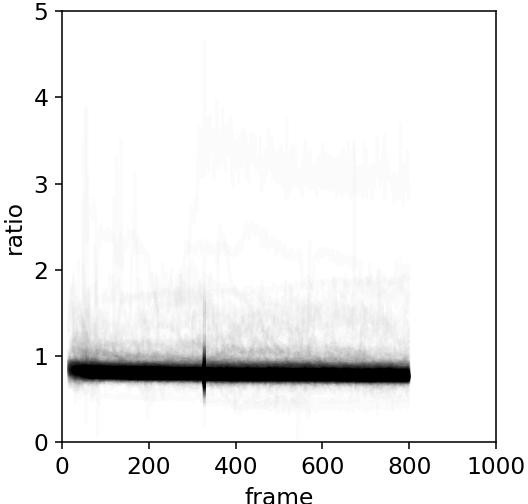
\includegraphics[width=\textwidth]{fig/all_cells_overlayed_mouse_neg}
	\end{subfigure}
	\hfill
	\begin{subfigure}{0.45\linewidth}
		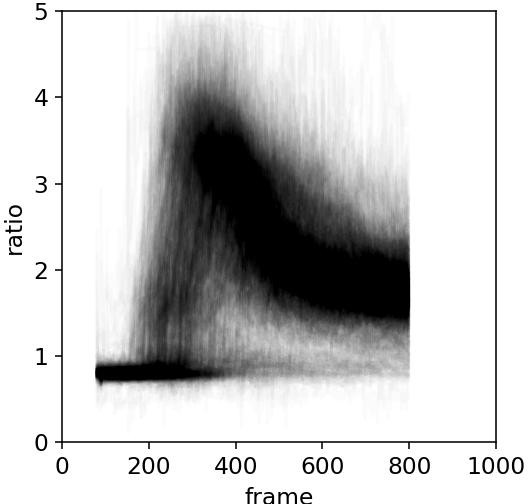
\includegraphics[width=\textwidth]{fig/all_cells_overlayed_mouse_pos}
	\end{subfigure}
	
	\caption{Two plots of the overlapping calcium concentration time series of cells. On the left a negative control and on the right a positive control of mouse cells.}
	\label{fig:all_cells_overlayed}
\end{figure}

By modelling the time series with a function incorporating features such as the increase, maximum value and oscillations present in the decrease afterwards, we can extract these features more easily. By doing this, using approximation methods from chapter~\ref{chapter:optimization}, we want to answer the research questions from the introduction.

From studying the data in the two control groups we find to expect a function close to
\begin{align}
	\label{math:function_unactivated_cell}
	f_{unac}(x) := u
\end{align}
for unactivated cells and
\begin{align}
	\label{math:function_activated_cell}
	f_{ac}(x) := \begin{cases}
		\frac{a-u}{1+ e^{-k(x-w)}} & \textbf{ if } x <= t\\
		\frac{d-f_{ac}(t)}{z-t} (x-t) + f_{ac}(t) & \textbf{ else}
	\end{cases}
\end{align}
for activated cells. The parameters can be understood as

\begin{table}[h!]
	\centering
	\begin{tabular}{|cl|}
		\hline
		$u$ ... & average value before activation, \\
		\hline
		$a$ ... & value reached at the peak of activation, \\
		\hline
		$k$ ... & steepness of increase, \\
		\hline
		$w$ ... & time point at which the increase happens, \\
		\hline
		$t$ ... & time point at which the increase ends, \\
		\hline
		$d$ ... & average value toward the end of the data, \\
		\hline
		$z$ ... & time point at which the data ends. \\
		\hline
	\end{tabular}
\end{table}

Figure~\ref{fig:typical_time_series_with_parameters} shows how the above functions~\ref{math:function_unactivated_cell} and~\ref{math:function_activated_cell} look and how the relations to the parameters are in unactivated and activated cells.

% u=0.9, a=4, k=0.075, w=300, t=400, d=2, z=800, f_ac(t)=3.098286
\begin{figure}
	\centering
	\begin{subfigure}{0.45\linewidth}
	  \begin{tikzpicture}
		\datavisualization [scientific axes, visualize as line,
			x axis = {
				min value = 0,
				max value = 1000,
				length = 5cm,
				ticks and grid = {major={at={0 as $t$}}, color=white},
				label = frame
			},
			y axis = {
				min value = 0,
				max value = 5,
				length = 5cm,
				ticks and grid = {major={at={0.9 as $u$}}},
				label = ratio
			},
		]
		data [format=function] {
			var x : interval [50:800]; func y = 0.9;
		};
	\end{tikzpicture}
	\end{subfigure}
	\hfill
	\begin{subfigure}{0.45\linewidth}
		\begin{tikzpicture}
			\datavisualization [scientific axes, visualize as line,
			x axis = {
				min value = 0,
				max value = 1000,
				length = 5cm,
				ticks and grid = {major={at={300 as $w$, 400 as $t$, 800 as $z$}}},
				label = frame
			}, y axis = {
				min value = 0,
				max value = 5,
				length = 5cm,
				ticks and grid = {major={at={0.9 as $u$, 2 as $d$, 4 as $a$}}},
				label = ratio
			},
			]
			data [separator=\space] {
				x y
				50 0.9000000223018123
				60 0.9000000472129365
				70 0.9000000999497857
				80 0.9000002115936903
				90 0.9000004479438116
				100 0.9000009482969035
				110 0.9000020075438745
				120 0.9000042499673413
				130 0.9000089971671542
				140 0.9000190469412669
				150 0.9000403220982461
				160 0.9000853606424553
				170 0.9001807029235496
				180 0.9003825231855573
				190 0.9008096899891967
				200 0.9017136137744631
				210 0.9036254818216721
				220 0.9076651317855678
				230 0.9161823896500311
				240 0.9340595221548389
				250 0.9712298467210794
				260 1.047020206850457
				270 1.1955833411872394
				280 1.4655191237997047
				290 1.8945460325562817
				300 2.45
				310 3.005453967443718
				320 3.434480876200295
				330 3.704416658812761
				340 3.8529797931495433
				350 3.9287701532789203
				360 3.9659404778451615
				370 3.983817610349969
				380 3.9923348682144324
				390 3.9963745181783277
			}
			data [format=function] {
				var x : interval [400:800]; func y = (2 - 3.998286) / (800 - 400) * (\value x - 400) + 3.998286;
			}
			info {
			\draw (visualization cs: x=300, y=2.45)
			node [left,font=\footnotesize] {$k$};
			};
		\end{tikzpicture}
	\end{subfigure}
	
	%3.1/(1 + exp(-0.075 * (\value x - 300))) + 0.9
	
	\caption{Left shows the function $f_{unac}$ defined in~\ref{math:function_unactivated_cell} with the parameter $u$. The right shows the function $f_{ac}$ defined in~\ref{math:function_activated_cell} with the parameters $u$, $d$, $a$, $w$, $t$, $z$ and $k$.}
	\label{fig:typical_time_series_with_parameters}
\end{figure}

For our model to make sense we have to impose some conditions onto the parameters. We expect $0 \leq u \leq d \leq a$, $w \leq t$ and $k > 0$.

There are multiple ways in which the parameters of $f_{ac}$ can be chosen to get a function similar to $f_{unac}$. If $w \gg z$ or $u \approx d \approx a$ then $f_{ac}$ approaches a constant value of $u$, thus approximating $f_{unac}$. If the approximation of a cell has parameters with $w \gg z$ or $u \approx d \approx a$ we can therefore expect it to be of an unactivated cell. Otherwise, it is more probable to be activated.

\section{Implementation}

Now that we have defined our model functions we will implement a routine that fits such a $f_{ac}$-function through the data of a cell.

main:
* read data
* filter data
* seperate single particles
* skip if too short
* approximate
* show approx and real data
* save parameters

approximate:
* set boundaries for parameters
* set start approx values for parameters
* scipy.optimize.curve-fit
* calculate approximation
* return paramters
